
\documentclass[12pt,letterpaper]{article}
\usepackage{graphicx,textcomp}
\usepackage{natbib}
\usepackage{setspace}
\usepackage{fullpage}
\usepackage{color}
\usepackage[reqno]{amsmath}
\usepackage{amsthm}
\usepackage{fancyvrb}
\usepackage{amssymb,enumerate}
\usepackage[all]{xy}
\usepackage{endnotes}
\usepackage{lscape}
\newtheorem{com}{Comment}
\usepackage{float}
\usepackage{hyperref}
\newtheorem{lem} {Lemma}
\newtheorem{prop}{Proposition}
\newtheorem{thm}{Theorem}
\newtheorem{defn}{Definition}
\newtheorem{cor}{Corollary}
\newtheorem{obs}{Observation}
\usepackage[compact]{titlesec}
\usepackage{dcolumn}
\usepackage{tikz}
\usetikzlibrary{arrows}
\usepackage{multirow}
\usepackage{xcolor}
\newcolumntype{.}{D{.}{.}{-1}}
\newcolumntype{d}[1]{D{.}{.}{#1}}
\definecolor{light-gray}{gray}{0.65}
\usepackage{url}
\usepackage{listings}
\usepackage{color}

\definecolor{codegreen}{rgb}{0,0.6,0}
\definecolor{codegray}{rgb}{0.5,0.5,0.5}
\definecolor{codepurple}{rgb}{0.58,0,0.82}
\definecolor{backcolour}{rgb}{0.95,0.95,0.92}

\lstdefinestyle{mystyle}{
	backgroundcolor=\color{backcolour},   
	commentstyle=\color{codegreen},
	keywordstyle=\color{magenta},
	numberstyle=\tiny\color{codegray},
	stringstyle=\color{codepurple},
	basicstyle=\footnotesize,
	breakatwhitespace=false,         
	breaklines=true,                 
	captionpos=b,                    
	keepspaces=true,                 
	numbers=left,                    
	numbersep=5pt,                  
	showspaces=false,                
	showstringspaces=false,
	showtabs=false,                  
	tabsize=2
}
\lstset{style=mystyle}
\newcommand{\Sref}[1]{Section~\ref{#1}}
\newtheorem{hyp}{Hypothesis}

\title{Problem Set 1}
\date{Due: September 30, 2024}
\author{Applied Stats/Quant Methods 1}

\begin{document}
	\maketitle
	
	\section*{Instructions}
	\begin{itemize}
		\item Please show your work! You may lose points by simply writing in the answer. If the problem requires you to execute commands in \texttt{R}, please include the code you used to get your answers. Please also include the \texttt{.R} file that contains your code. If you are not sure if work needs to be shown for a particular problem, please ask.
		\item Your homework should be submitted electronically on GitHub.
		\item This problem set is due before 23:59 on Monday September 30, 2024. No late assignments will be accepted.
		%\item Total available points for this homework is 80.
	\end{itemize}
	
	\vspace{1cm}
	\section*{Question 1: Education}
	
	A school counselor was curious about the average of IQ of the students in her school and took a random sample of 25 students' IQ scores. The following is the data set:\\
	\vspace{.5cm}
	
	\lstinputlisting[language=R, firstline=36, lastline=36]{my_answer_YuFan.R}  
	
	\vspace{1cm}
	
	\begin{enumerate}
		\item Find a 90\% confidence interval for the average student IQ in the school.\\
		\lstinputlisting[language=R, firstline=39, lastline=46]{my_answer_YuFan.R}
		
		\item Next, the school counselor was curious  whether  the average student IQ in her school is higher than the average IQ score (100) among all the schools in the country.\\ 
		\noindent Using the same sample, conduct the appropriate hypothesis test with $\alpha=0.05$.
		
		\lstinputlisting[language=R, firstline=53, lastline=59]{my_answer_YuFan.R}  
	\end{enumerate}
	
	\newpage
	
	\section*{Question 2: Political Economy}
	
	\noindent Researchers are curious about what affects the amount of money communities spend on addressing homelessness. The following variables constitute our data set about social welfare expenditures in the USA. \\
	\vspace{.5cm}
	
	
	\begin{tabular}{r|l}
		\texttt{State} &\emph{50 states in US} \\
		\texttt{Y} & \emph{per capita expenditure on shelters/housing assistance in state}\\
		\texttt{X1} &\emph{per capita personal income in state} \\
		\texttt{X2} &  \emph{Number of residents per 100,000 that are "financially insecure" in state}\\
		\texttt{X3} &  \emph{Number of people per thousand residing in urban areas in state} \\
		\texttt{Region} &  \emph{1=Northeast, 2= North Central, 3= South, 4=West} \\
	\end{tabular}
	
	\vspace{.5cm}
	\noindent Explore the \texttt{expenditure} data set and import data into \texttt{R}.
	\vspace{.5cm}
	\begin{itemize}
		
		\item
		Please plot the relationships among \emph{Y}, \emph{X1}, \emph{X2}, and \emph{X3}? What are the correlations among them (you just need to describe the graph and the relationships among them)?
		
		\lstinputlisting[language=R, firstline=65, lastline=75]{my_answer_YuFan.R}
		\begin{verbatim}
			STATE                 Y                X1             X2              X3       
			Length:50          Min.   : 42.00   Min.   :1053   Min.   :111.0   Min.   :326.0  
			Class :character   1st Qu.: 67.25   1st Qu.:1698   1st Qu.:187.2   1st Qu.:426.2  
			Mode  :character   Median : 79.00   Median :1897   Median :241.5   Median :568.0  
			Mean   : 79.54   Mean   :1912   Mean   :281.8   Mean   :561.7  
			3rd Qu.: 90.00   3rd Qu.:2096   3rd Qu.:391.8   3rd Qu.:661.2  
			Max.   :129.00   Max.   :2817   Max.   :531.0   Max.   :899.0 
		\end{verbatim} 
		\lstinputlisting[language=R, firstline=77, lastline=80]{my_answer_YuFan.R}  
		\begin{verbatim}
			Y        X1        X2        X3
			Y  1.0000000 0.5317212 0.4482876 0.4636787
			X1 0.5317212 1.0000000 0.2056101 0.5952504
			X2 0.4482876 0.2056101 1.0000000 0.2210149
			X3 0.4636787 0.5952504 0.2210149 1.0000000
		\end{verbatim} 
		
		The correlation coefficient between Y and X1 is 0.5317212, indicating a moderate positive correlation.\\
		
		The correlation coefficient between Y and X2 is 0.4482876, indicating a slight to moderate positive correlation.\\
		
		The correlation coefficient between Y and X3 is 0.4636787, indicating that they have a slightly higher positive correlation than Y and X2.\\
		
		The correlation coefficient between X1 and X2 is 0.2056101, indicating a weak positive correlation.\\
		
		The correlation coefficient between X1 and X3 is 0.5952504, indicating a moderate positive correlation.\\
		
		The correlation coefficient between X2 and X3 is 0.2210149, indicating a weak positive correlation.\\
		
		\lstinputlisting[language=R, firstline=82, lastline=86]{my_answer_YuFan.R}  
		
		\begin{enumerate}
			\item[]
			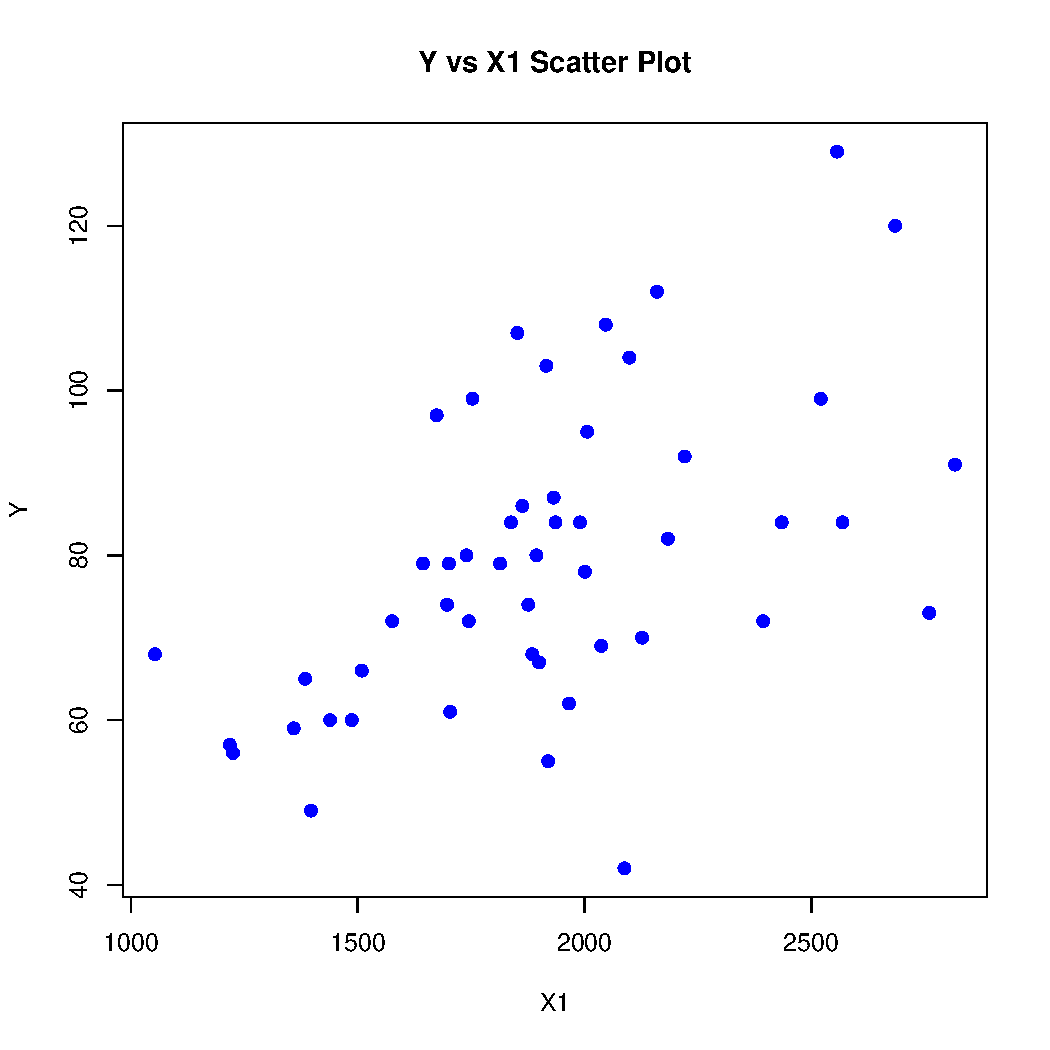
\includegraphics[width=.85\textwidth]{plot.Y.X1_YuFan.pdf}
		\end{enumerate}   
		
		\lstinputlisting[language=R, firstline=88, lastline=92]{my_answer_YuFan.R}  
		\begin{enumerate}
			\item[]
			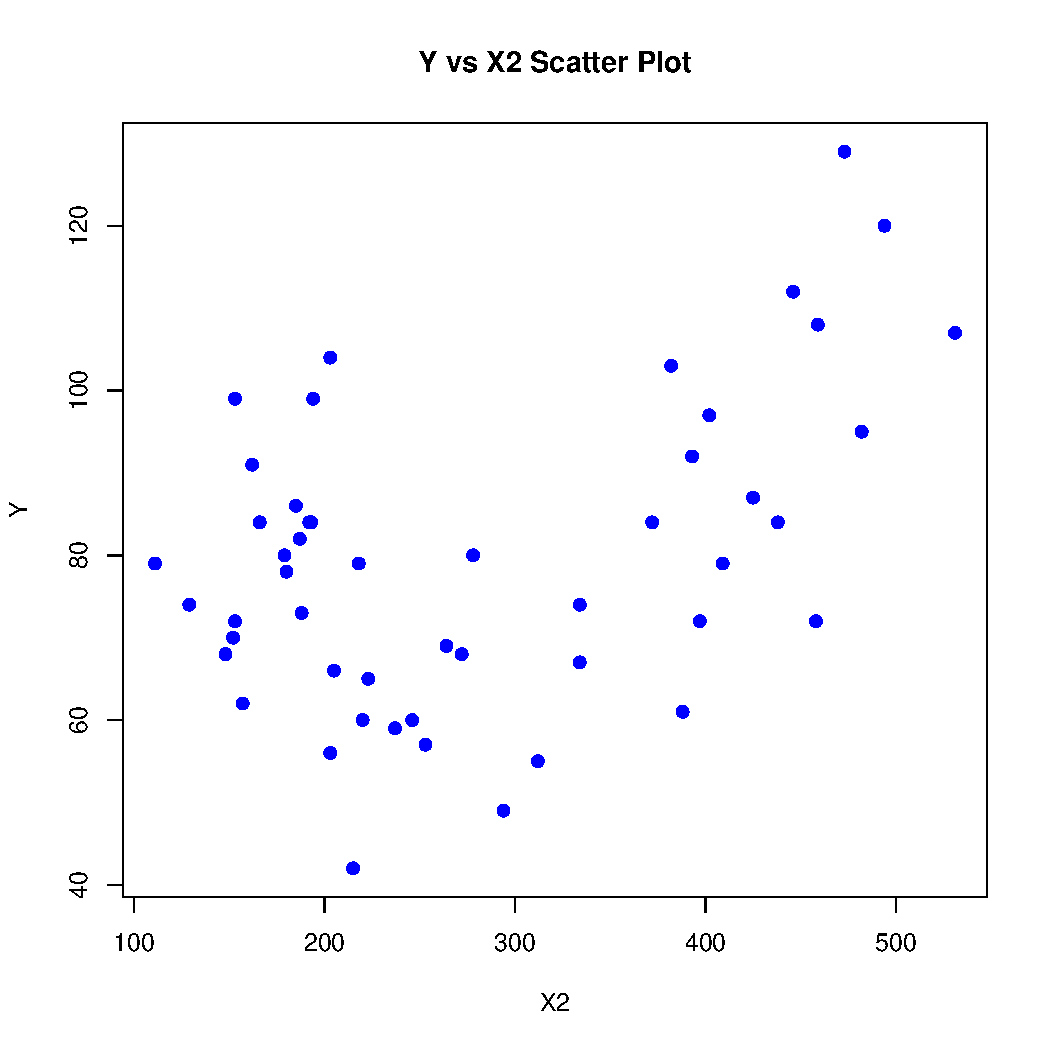
\includegraphics[width=.85\textwidth]{plot.Y.X2_YuFan.pdf}
		\end{enumerate}   
		
		\lstinputlisting[language=R, firstline=94, lastline=98]{my_answer_YuFan.R}  
		\begin{enumerate}
			\item[]
			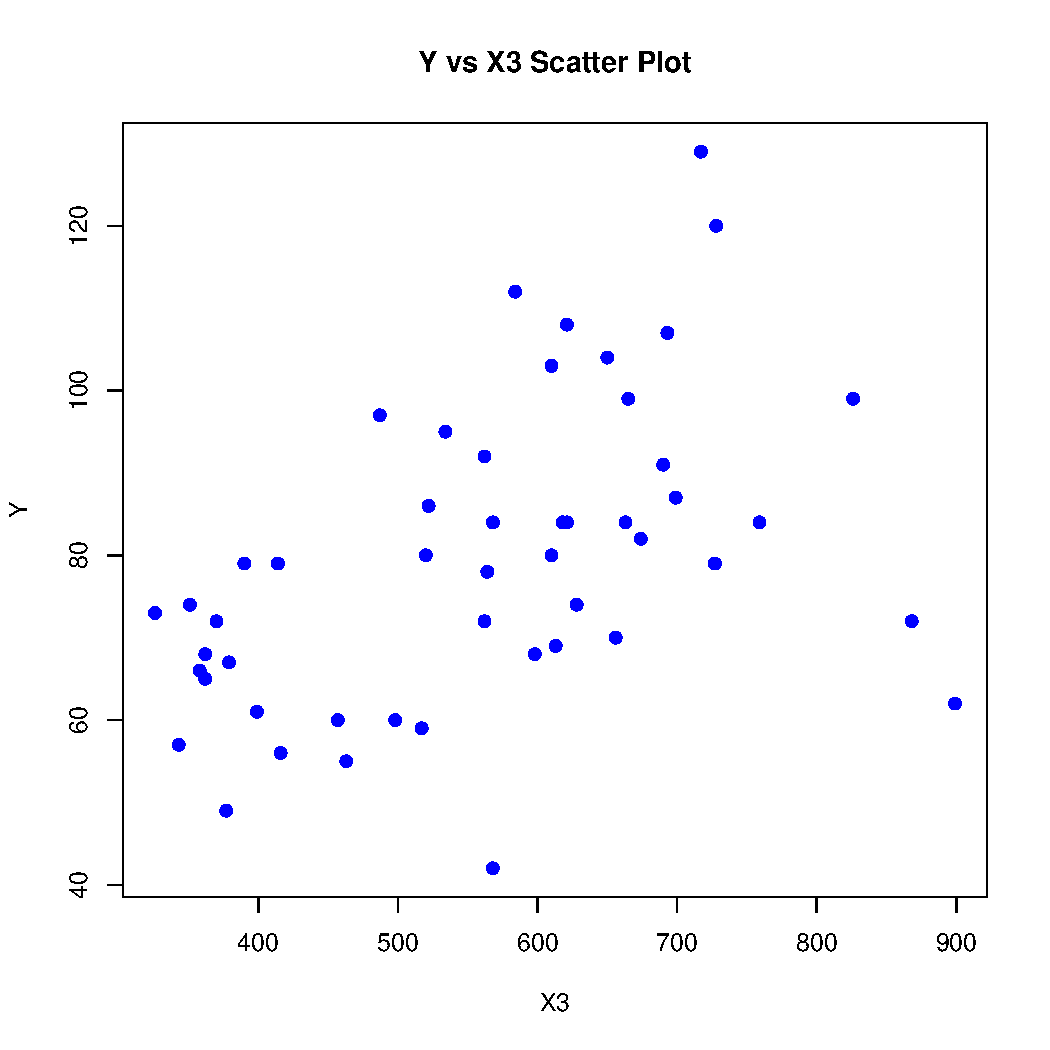
\includegraphics[width=.85\textwidth]{plot.Y.X3_YuFan.pdf}
		\end{enumerate} 
		
		\lstinputlisting[language=R, firstline=100, lastline=104]{my_answer_YuFan.R}  
		\begin{enumerate}
			\item[]
			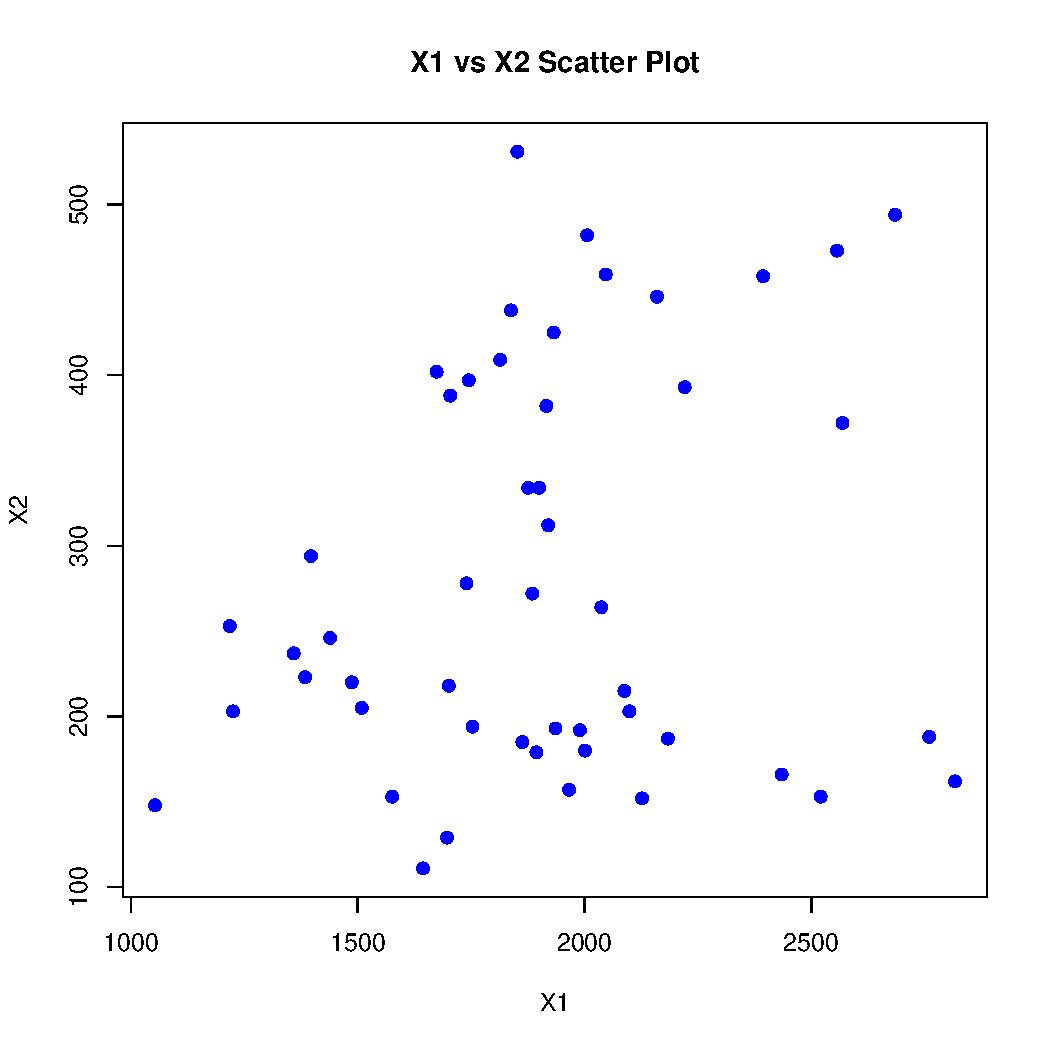
\includegraphics[width=.85\textwidth]{plot.X1.X2_YuFan.pdf}
		\end{enumerate} 
		
		\lstinputlisting[language=R, firstline=106, lastline=110]{my_answer_YuFan.R}  
		\begin{enumerate}
			\item[]
			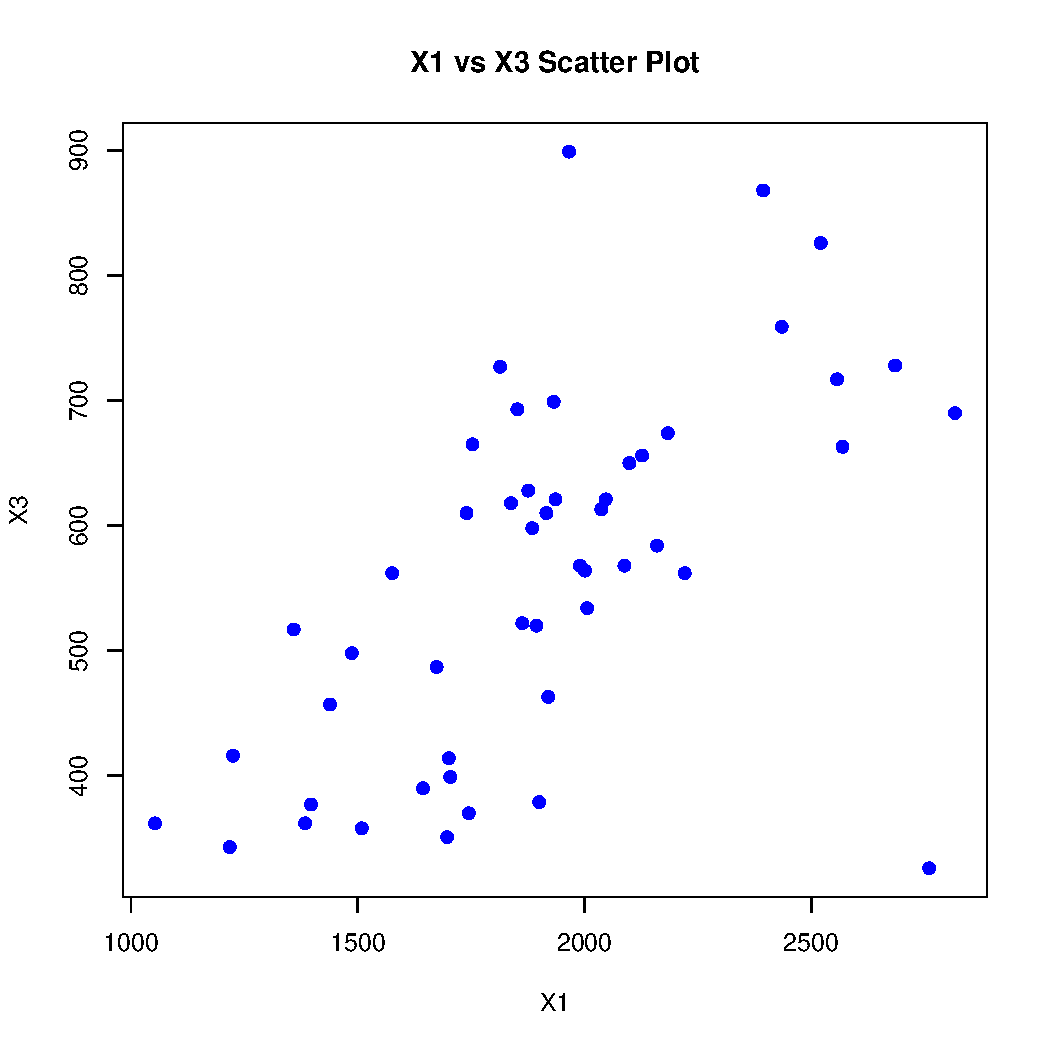
\includegraphics[width=.85\textwidth]{plot.X1.X3_YuFan.pdf}
		\end{enumerate} 
		
		\lstinputlisting[language=R, firstline=112, lastline=116]{my_answer_YuFan.R}  
		\begin{enumerate}
			\item[]
			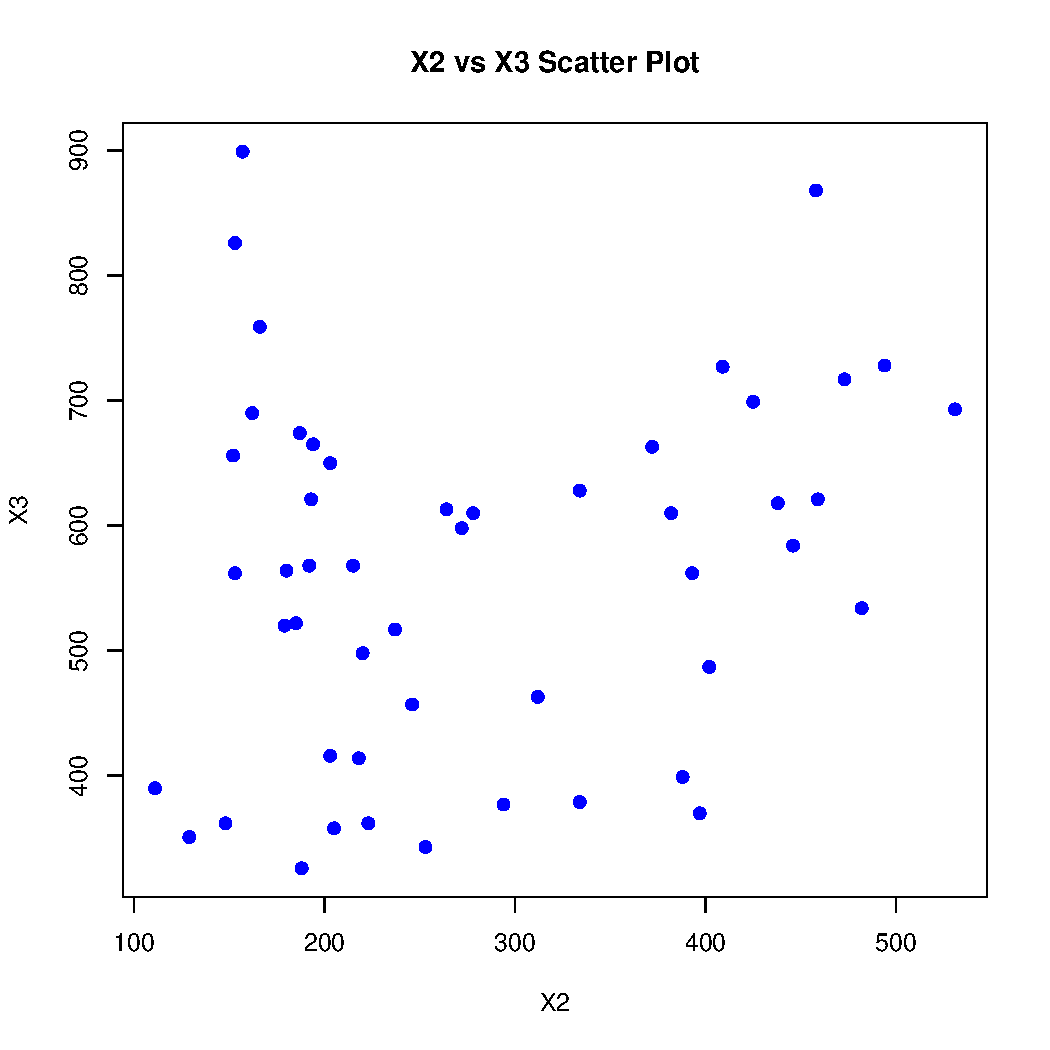
\includegraphics[width=.85\textwidth]{plot.X2.X3_YuFan.pdf}
		\end{enumerate} 
		
		\newpage
		
		\item
		Please plot the relationship between \emph{Y} and \emph{Region}? On average, which region has the highest per capita expenditure on housing assistance?
		
		\lstinputlisting[language=R, firstline=119, lastline=128]{my_answer_YuFan.R}
		\begin{enumerate}
			\item[]
			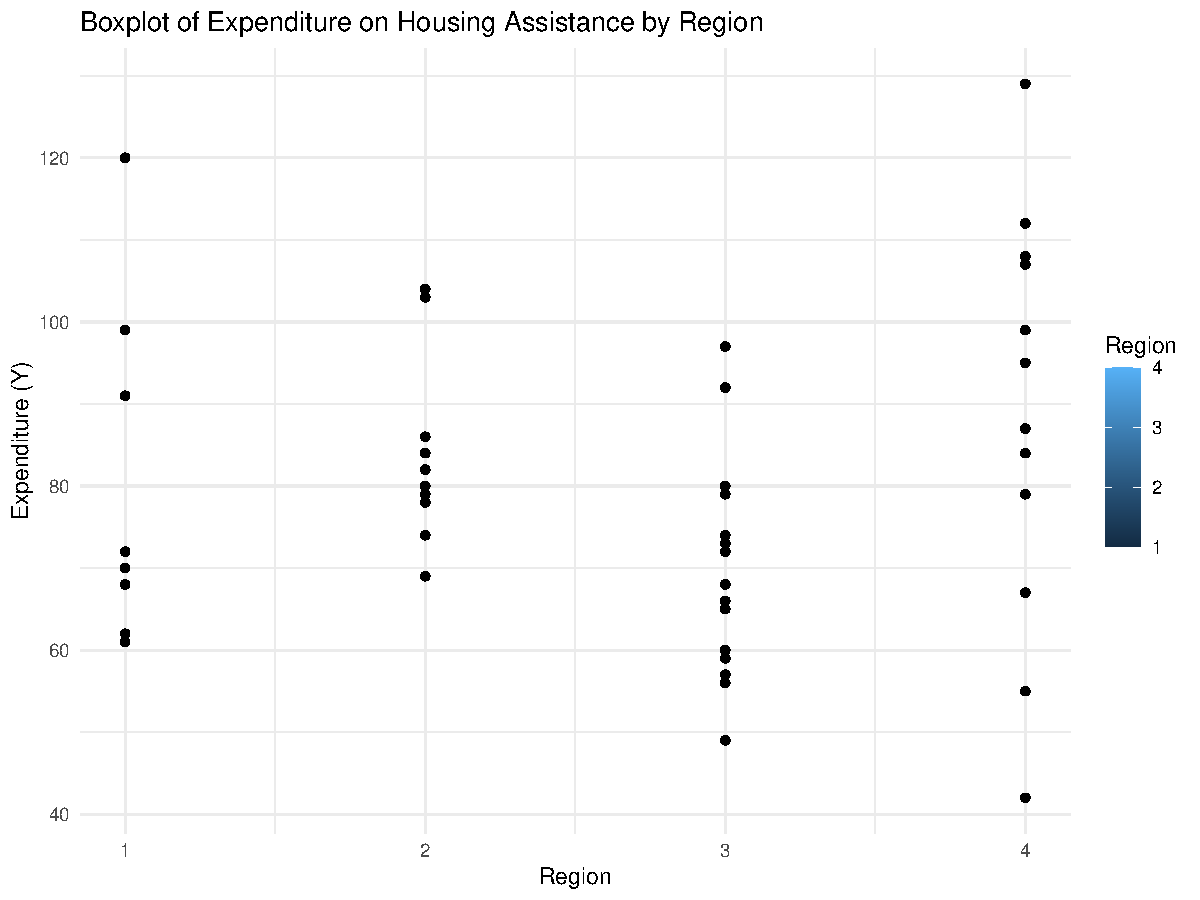
\includegraphics[width=.85\textwidth]{boxplot.Y.Region_YuFan.pdf}
		\end{enumerate}
		
		\lstinputlisting[language=R, firstline=131, lastline=138]{my_answer_YuFan.R}
		\begin{figure}
			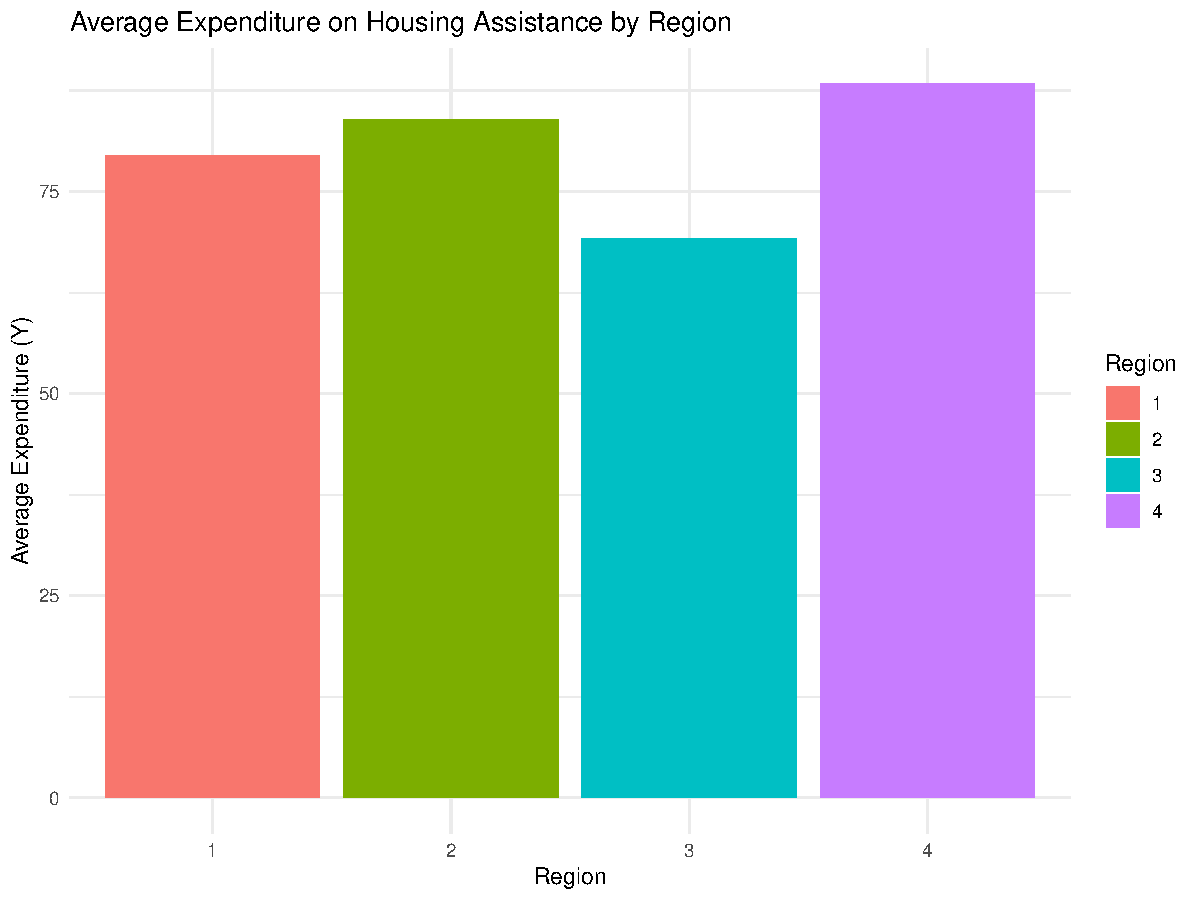
\includegraphics[width=.85\textwidth]{barplot.Y.Region_YuFan.pdf}
		\end{figure}
		
		As can be seen from the bar chart, per capita expenditure on housing benefit is highest in region 4\\
		
		\vspace{.5cm}
		
		\item
		Please plot the relationship between \emph{Y} and \emph{X1}? Describe this graph and the relationship. Reproduce the above graph including one more variable \emph{Region} and display different regions with different types of symbols and colors.
		
		\lstinputlisting[language=R, firstline=141, lastline=152]{my_answer_YuFan.R}
		
		\begin{figure}
			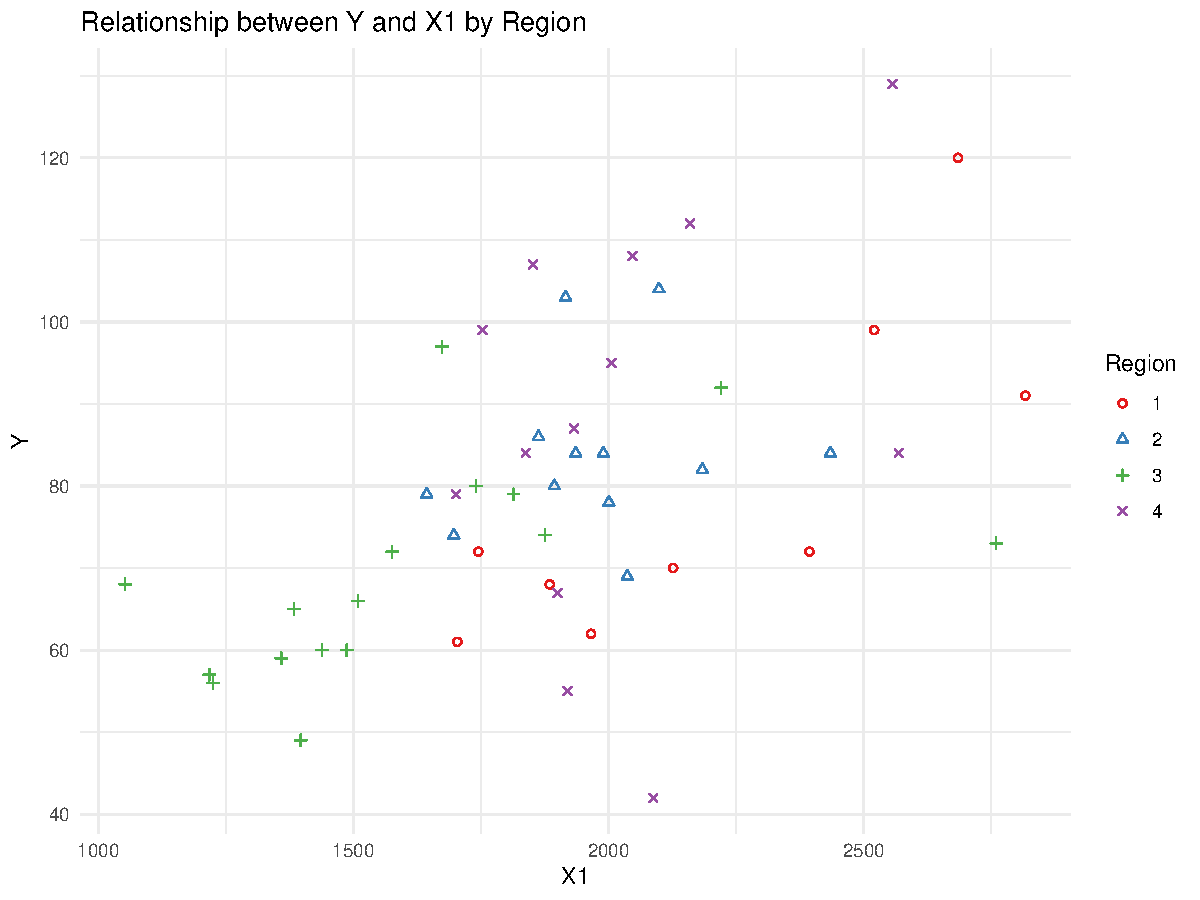
\includegraphics[width=.85\textwidth]{plot_Y_X1_by_Region.pdf}
		\end{figure}
		
	\end{itemize}
	
	
\end{document}